\chapter{Problem Statement}

From the beginning of civilization, humans have been looking to transport from one place to another more efficiently than walking. First, they started with horses and floats, but horses had a brain and could make their own decisions; sometimes, those decisions were based on an emotional reaction rather than intelligent choices. Moreover, it could not continuously work for a long duty cycle, and its power was limited. Later in 1769, Nicolas-Joseph Cugnot invented the first steam-powered vehicle. This incredible machine could load an extended weight, and drivers could make their own driving decisions. Until now, this transportation system is still working, unless the advantage of efficiency, power consumption, pollution, and safety is not enough to be an optimal way to transport people and loads.\\

Research areas have made many efforts to achieve an optimal way of transportation to be accessible, optimal, and safe for everybody. Some ideas have been proposed, like hydrogen, diesel, and natural gas engines. Also, some Nobel research about control safety systems like better and more powerful breaks, automated airbags, and good chassis material tries to save more lives, but it is not enough. Unfortunately, all past advantages are focused on the driver and vehicle users. Currently, no control system guarantees the security and integrity of the other road authors. The human decision in a driving context frequently represents a danger because it is based on emotion and natural reactions making no optimal driving. Even though these options could improve the current vehicles, they may find a better and cheapest solution to the main problem.\\

The research areas try to solve the safety driving problem with deep learning, Recurrent Neural Networks, machine learning, and other theories. However, using these theories only guarantees stability and controllability in some scenarios. To get a closer solution to this problem, we study one way of achieving security and efficiency in a particular method as a highway area in this thesis work. Currently, the experts on optimal control system areas rely on automated driving. This technology could solve all of the problems mentioned above.\\

Some safety decision criteria that we take into account were the following:
\begin{itemize}
\item Avoid obstacles that may be on the road.
\item Avoid a collision with other cars on the road regardless of whether it is a cooperative or non-cooperative agent.
\item Make decisions in the presence of aggressive maneuvers by selfish or non-cooperative agents on the road.

\end{itemize}


Therefore, designing and implementing different controllers with access to specific data sets was necessary. It depends on each controller's necessity. These decisions are based on logical and optimal decision-maker control to achieve the desired goal.

 These decisions are based on safety rules established for the users of any particular road.


% --------------------- automated driving --------------------
\section{Automated driving}
The idea of automated driving is to safely and efficiently coordinate and synchronize several autonomous vehicles (AV) safely and efficiently.\\

Managing many AVs requires an extensive network with high computational loads and advanced control techniques. Usually, in the research literature is implemented one control algorithm is for an agent to achieve the objective. However, automated driving is an area that must consider different scenarios and situations. Besides, it is essential to prove all possibilities for warranty security and controllability. This thesis studies some control theories and the best state to implement.

\begin{itemize}
    \item  \textbf{Mixed-Integer Potential Game:} uses integer and continuous variables in a cost function to control the AV's position and velocity on a highway optimally.
    \item  \textbf{Model Predictive Control:} uses information about the environment and local variables to get the optimal decision avoiding near obstacles.
    \item  \textbf{Alternating Direction Method of Multipliers:} utilize a linear model of the AV and inequality constraints as possible to get a faster and more efficient solution to the problem. 
\end{itemize}

All the above controllers are explained in detail in chapter 4. In addition, the following section describes how AV and collision avoidance are modeled. 






% -----------------------------------------
\section{Vehicle Model}

The automated driving task is complex, and one model is not enough to represent the behaviour of a vehicle around the environment. However, multiple controllers require multiple models that give the correct information. We use three different controllers that have a specific task. Each of them needs a particular model of vehicle. The high-level controller takes the network's information. For that reason, we implement a linear model. The middle-level controller uses just the knowledge of the environment acquired by its sensors. Due to this reason, we implemented a unicycle model. Besides, the low-level control gets information about the car and its decision-making behavior. Thus, we use a differential model in this control section. 


% -----------------------------------------
\subsection{Linear Model System}
\label{linear_model_system}

For controllers based on game theory, convexity is the main prerequisite for convergence. Therefore, the robot model and its constraints must be linear and convex. Due to this, the system is based on a Mixed-Logical-Dynamical system \cite{BEMPORAD1999407}. We consider a set of vehicles $\mathcal{I}:= \left \{ 1, ..., N \right \}$ where N is the total number of vehicles interacting with the local agent in a multi-lane environment. The set  $\mathcal{L}:= \left \{ 1, ..., L \right \}$ represents the set of current lines on the highway, and the L variable is the maximum number of lines on the way. We assume that each vehicle $i$ can control its longitudinal speed $v_i \in \mathcal{V}_i \subset \mathbb{R}$  and can change lane $z_i \in \mathcal{L} \subset \mathbb{N}$. Over the prediction horizon $\mathcal{T} := \left \{ 0, ... ,T \right \} , T\geq 1$. We use two different decision variables to better represent an AV on a highway. Mixed logical variables can simplify, make linear, and convex the entire system. 

\begin{figure}[H]
    \centering
    \includegraphics[width=0.8\textwidth]{Kap3/linear_model.png}
    \caption{Linear model's variables.}
    \label{fig:variables}
\end{figure}


\subsubsection{Continuous Decision Variables}
\label{continous_decision_variables}

Each vehicle model has continues variables that represent some physical features. Longitudinal acceleration $a_i \in A_i := \left [ \underline{a_i}, \overline{a_i} \right ] \subset \mathbb{R}$, the variables $\left \{ \underline{a_i}, \overline{a_i} \right \}
$ represent the minimum and maximum acceleration allowed, with $\underline{a_i}< 0 <  \overline{a_i} $, assuming that the $\underline{a_i}$ is negative and is due the break job of the $i$ vehicle, as illustrated in Fig. \label{fig:variables}. The longitudinal speed $v_i \in \mathcal{V}_i \subset \mathbb{R}$ is determined by a standard Forward-Euler Scheme, i.e.,

\begin{gather}
v_i(t+1) = v_i(t) + \tau a_i(t),
\end{gather}

where $\tau > 0$ denotes the time interval of each simulation step. Hence, the acceleration and velocity longitudinal over the horizon $\mathcal{T}$ are: 
\begin{gather*}
a_i := \left [ a_i(0); ...; a_i(t-1) \right ] \in \mathcal{A}^T_i, \\
v_i := \left [ v_i(0); ...; v_i(t-1) \right ] \in \mathcal{V}^T_i
\end{gather*}




\subsubsection{Discrete Decision Variables}
\label{discrete_decision_variables}
The lanes in a highway are predefined internationally as a space where vehicles can and should travel. Thanks to this design, the agent will drive inside a lane unless the vehicle needs to change to another one. That means the set of vehicles $\mathcal{V}$ needs to be modelled as an integer variable that represents the actual and future travelling lane $z_i \in \mathcal{L}$. The discrete decision variables over the horizon $\matchal{T}$ are:

\begin{gather*}
z_i := \left [ z_i(0); ...; \ z_i(t-1) \right ] \in \mathcal{Z}^T_i.
\end{gather*}



\subsubsection{Coupling Variables}



The control system requires different sense variables that allow knowing the actual and future states of the agent $i$ with its neighbours $\mathcal{I}_{-i}$. Therefore, we denote by $d_{i,j} \in \mathbb{R}$ as the longitudinal distance between the connected vehicles $i$ and $j$ at the time $t \in \mathcal{L}$ as shown the Fig. \ref{fig:distance}. 



\begin{figure}[H]
    \centering
    \includegraphics[width=0.7\textwidth]{Kap3/Asset 4.png}
    \caption{Relative distance between agents.}
    \label{fig:distance}
\end{figure}


Over time, the equation of $d_{i,j}$ evolves as a Forward-Euler function. In Eq. \ref{eq:distance} the longitudinal distance is over the axis $x$ in the working environment. The difference in distance velocities is over the current time $t$, and the $\tau$  delta time is the controller's step time for each iteration.

\begin{equation}
d_{i,j}(t+1)= d_{i,j}(t) + \tau(v_j(t)-v_i(t)).
\label{eq:distance}
\end{equation}



It allows us to introduce the set of vehicles in the neighbourhood of  $\mathcal{N}_i:= \left\{ j \in \mathcal{I}  | \left| d_{i,j} \right| \le \overline{d}, t \in \mathcal{T}\right\}$; this data can be measured locally or globally example, on the on-board sensors or with communication of a driving network. From now we refer to the variable $j$ as a generic vehicle in the set $\mathcal{N}_i$. According to \label{eq:distance}, each agent knowing the velocity of its neighbour $v_j(t)$, can estimate the relative distance between each other.
In addition, we implement a relative lane distance $z_{i,j}$. It represents the lateral distance of each vehicle from its neighbours. The difference of lane between agent $i$ with its neighbors $\mathcal{N}_i$ and is calculated by the following equation:



\begin{equation}
z_{i,j}(t)= z_{j}(t) - z_{i}(t).
\label{eq:lanes}
\end{equation}



Lateral distance is the difference between integer values. It means the space working is $\mathbf{N} \times \mathbf{N} \to \mathbf{N}$. The distance is calculated over the $y$ axis.


\begin{figure}[H]
    \centering
    \includegraphics[width=0.8\textwidth]{Kap3/Asset 5.png}
    \caption{Lateral Distance.}
    \label{fig:lanes}
\end{figure}

We assume that each agent makes decisions for their selfish interest, e.g., drive through desired speed profile $v_i^d \in \mathcal{V}^T_i$ or get into a lane $z_i^d \in \mathcal{L}^T_i $. Each agent's control system takes into account its neighbours' current and future state. Still, it does not provide information about the targets of the other agents. As a result of this behaviour, each agent takes a decision seeking its individual goals through a sequence of hybrid decisions.
With the previous model, we formulate as a first step a Model Predictive Control (MPC) motion planning with mixed-integer variables:

\begin{align}
\left\{ \begin{matrix}
\begin{aligned}
 \min_{v_i, a_i, z_i} & J_i(v_i, a_i, z_i) & \\
\text{s.t.} \quad & v_i(t+1)=v_i(t)+ \tau \ a_i(t), & \forall t \in \mathcal{T} \\
& a_i(t) \in \mathcal{A}_i,  &   \\
 & v_i(t+1) \in \mathcal{V}_i,  &   \\
 & z_i(t+1) \in \mathcal{L}_i,  &   \\
\end{aligned}
\end{matrix} \right.
\label{eq:MPC1}
\end{align}


% \begin{align}
% \left\{\begin{matrix}
% \begin{aligned}
% \min_{v,a,z, l_i^l,l_i^r} \quad & J_i\left ( v_i, a_i, z_i \right )\\
% \textrm{s.t.} \quad & v_i(t+1) = v_i(t)+\tau a_i(t), & \forall t \in \mathcal{T}\\
%   &   z_i(t+1) = z_i(t) + l_i^l(t) - l_i^r(t),  & \forall t \in \mathcal{T} \\
% & a_i(t) \in \mathcal{A} , & \forall t \in \mathcal{T} \\
% & v_i(t) \in \mathcal{V_i} , & \forall t \in \mathcal{T} \\
% & a_i(z) \in \mathcal{L_i} , & \forall t \in \mathcal{T} \\
% &  l_i^l(t),l_i^r(t)\in \mathbb{B},  & \forall t \in \mathcal{T} \\
% & l_i^l(t) + l_i^r(t)  \leq 1, & \forall t \in \mathcal{T}\\
% & (\text{\ref{eq:4_6real}}) - (\text{\ref{eq:4_20}}) . & \forall j \in \mathcal{N}_i, \forall t \in \mathcal{T} 
% \end{aligned}
% \end{matrix}\right.
% \label{eq:MPC_problem}
% \end{align}


\\
The $J_i$ cost function is a linear and convex objective for each vehicle $i$ where $J_i:\mathcal{V}^T_i \times \mathcal{A}^T_i \times  \mathcal{L}^T_i \longrightarrow  \mathbb{R}$. The sets $\mathcal{V}_i$ and $\mathcal{L}_i \subset \mathcal{L}$ shall be defined to restrict them to possible values in the real environment. Given maximum and minimum acceleration $\left[ \underline{a_i}, \overline{a_i} \right]$ as also maximum and minimum Velocity $\left[ \underline{v_i}, \overline{v_i} \right]$, we can limit the sets as:

\begin{align}
    \mathcal{V}_i(t) & :=\left[ 0,\overline{v_i(t)} \right] \cap \left[ v_i(t)+ \tau  \underline{a_i},\quad v_i(t)+ \tau  \overline{a_i} \right]
    \label{eq:set_v}
\\
    \mathcal{L}_i(t) & :=\mathcal{L} \cap \left[ z_i(t) -1, \quad z_i(t)+1 \right]
    \label{eq:set_z}
\end{align}

From \ref{eq:set_v}, it is possible to limit the speed to legally possible values, and from \ref{eq:set_z} limits the change of lane to just one per step. This restriction makes agents' movement smoother through lanes and allows lateral safety rules. The following section explains the rules to make safer automated driving with selfish agents.

\subsubsection{Collision Avoidance Rules}
 
Human driving is usually unsafe; exist some rules established in each country, like speed limits, preferential lanes, and safety distance. In this section, we postulate some safety rules to avoid the collisions of the interconnected agents with the presence of non-cooperative agents.\\

% -----------------------------------------------------------------------------
\subsubsection{Longitudinal rules}
The main reason for a collision of two or more vehicles is that one of the vehicles violates the safety distance. Due to this is implemented the following safety rule. If the lateral distance between two agents is equal to zero $z_j(t)=z_i(t) $ and the longitudinal distance is greater or less than a safety distance $\left| d_{i,j}(t) \right| > D_s$, and the agents will continue in the same lane $z_i(t+1) =  z_i(t), z_j(t+1) =  z_j(t)$. The control system must ensure that the behind vehicle maintains a safety distance $\left| d_{i,j}(t) \right| > D_s$ how is shown in Algorithm \ref{alg:safety}, where $D_s$ is a predefined secure distance.\\

\begin{algorithm}
\caption{Algorithm of longitudinal distance}\label{alg:safety}
\begin{algorithmic}
% \FOR $i \in \mathcal{V}$
% \FOR \forall {$i \in \mathcal{V}$} 
\If{$z_{i,j}(t)=0$ and $z_{i,j}(t+1) =0$}
    \If{$d_{i,j}(t) > 0 $}
        \State $d_j(v_j(t)) -d_i(v_i(t)) > D_s$
    \ElsIf{ $d_{i,j}(t) < 0$} 
        \State $d_j(v_j(t)) -d_i(v_i(t)) < -D_s$
    \Else
        
        \State Continue normal driving
    \EndIf
\EndIf

\end{algorithmic}
\end{algorithm}

% ----------------------------------------------------------------------------
\subsubsection{Lateral rules}

\begin{figure}
\begin{subfigure}[H]{1\textwidth}
\centering
    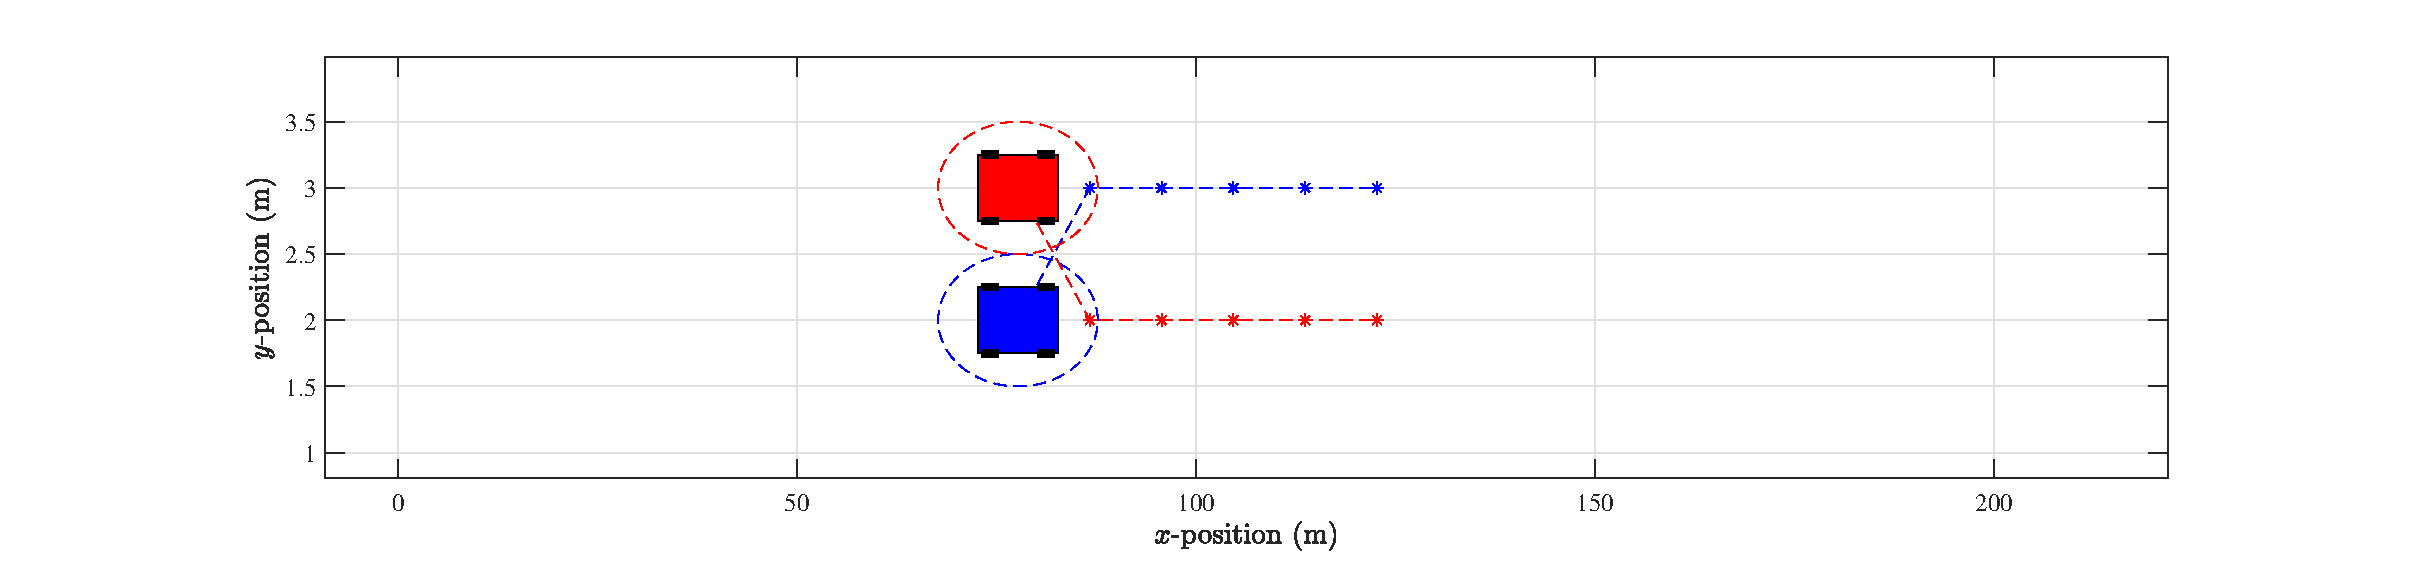
\includegraphics[width=0.95\textwidth]{Kap3/untitled.eps}
    \label{fig:lat_col1}
    \caption{Position of vehicles during the example.}
\end{subfigure}%
\vspace{1cm}
\begin{subfigure}[b]{1\textwidth}
\centering
    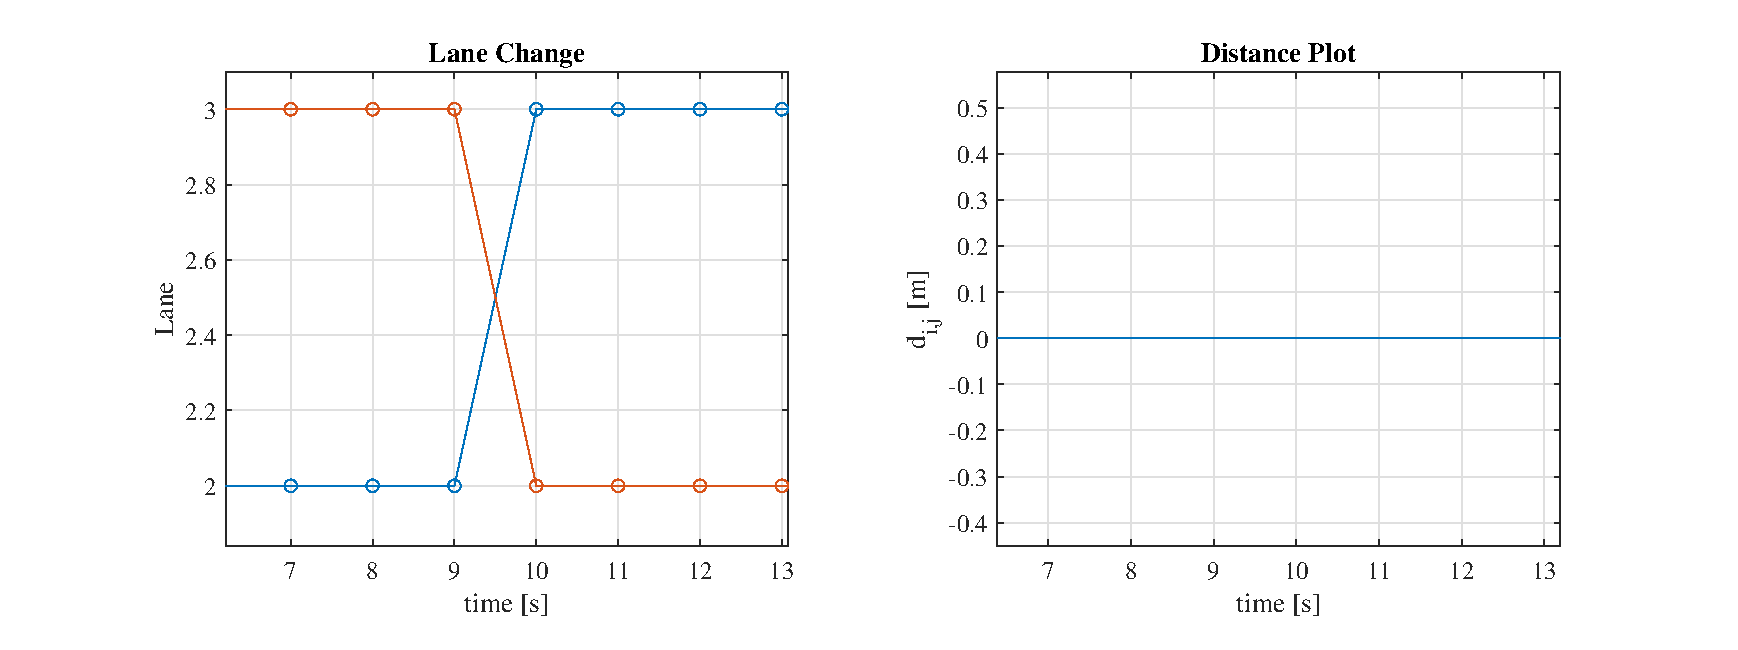
\includegraphics[width=0.95\textwidth]{Kap3/plot_change_line.eps}
    \caption{ Profiles of velocity and lanes over highway.}
    \label{fig:lat_col2}
\end{subfigure}
% \hfill
\caption{  Example of lateral collision.  }
\label{fig:lat_col}
\end{figure}

There are other common collisions in a regular lane; those are lateral collisions, usually generated by occlusion problems. This model does not have this issue thanks to interconnected and full neighbour position knowledge. However, the controller solver could be in a position where each vehicle decides to change at the same time the lane as Fig \ref{fig:lat_col} shows. Owing to this, we implement the lateral rule for each vehicle $i,j$ driving over the horizon $\mathcal{T}$, if the longitudinal distance $d_{i,j}$ is less than a safe distance and the difference of lane position $z_{i,j}$ is one $\left| z_{i,j} (t) \right|=1$, and the pair of agents will change the lane $z_{i} (t+1) \neq z_{i} (t), z_{j} (t+1) \neq z_{j} (t)$, the controller must constraint the change of lane as is explained in the next algorithm.

\begin{algorithm}
\caption{Algorithm of lateral distance}\label{alg:lat_saf}
\begin{algorithmic}
% \FOR $i \in \mathcal{V}$
% \FOR \forall {$i \in \mathcal{V}$} 
\If{ $\left| z_{i,j} (t) \right|=1$ and ($z_{i} (t+1) \neq z_{i} (t)$ or $ z_{j} (t+1) \neq z_{j} (t)$)}
    \If{$d_{i,j}(t) > 0 $}
        \State $d_j(v_j(t)) -d_i(v_i(t)) > D_s$
    \ElsIf{ $d_{i,j}(t) < 0$} 
        \State $d_j(v_j(t)) -d_i(v_i(t)) < -D_s$
    \Else
        
        \State Continue normal driving
    \EndIf
\EndIf

\end{algorithmic}
\end{algorithm}

Finally,  the previous safety rules are executed in a mixed-integer decision-making framework explained in-depth way in chapter \ref{nonlinear_model}. Nevertheless, this thesis work does not focus on the issue of communication among vehicles. Consequently, we assume that:
\begin{itemize}
\item Vehicles can share data of their position, speed, current lane and future states planned. 
\item Each vehicle is autonomous, therefore it has the capability to change its position and velocity without the presence or intervention of a human being
\end{itemize}








% \section{Robot Architecture}
% //////////////////////////////////////////////////////

% ##############################################


\subsection{Non-Linear Model System}
\label{nonlinear_model}
Currently, there are several kinds of wheel robots used for mobile applications. Some of them are unicycle, Ackerman, differential, and omnidirectional, among others. In \cite{81t} was compared the two main ways to represent a dynamic system and the kinetic and kinematic models were compared in the vehicle collision avoidance framework. Although the kinetic model has more accuracy than the kinematic, the entire system implemented in an MPC is faster with the kinematic model than with the kinetic model. Due to better prediction accuracy and computational time in the established prediction horizon, we decided to use the robot's kinematic model. 
\\
The nonlinear kinematic unicycle model is one of the most popular models for automated driving in multiagent systems \cite{kinematic} and mobile robotics. Therefore, we designed, fine-tuned, manufactured and implemented a linear unicycle model for the medium level of control. It makes the following assumptions:


\begin{itemize}
    \item Into the prediction horizon of the MPC., the velocity V could change.
    \item Forces are applied only in the lateral wheels, neither in the caster wheels.
    \item The robot is not equipped with a steering wheel.
    \item Aerodynamic drag and rolling resistance are ignored.
    \item The position of the front and rear caster wheel does not matter.
    \item The Center of Gravity (CG) position is assumed in the middle of the lateral wheels; the height is assumed to be zero since the vehicle's motion is planar.
    \item Pitch and roll dynamics are neglected. 
    \item The electrical energy and forces applied to the traction wheels are neglected.
\end{itemize}
\\

In order to specify the actual position of the robot within two-dimensional space, we use a relationship between the robot's global reference and the robot's local reference, as shown in Fig \ref{kinematic2}. The Axis X and Y define the position related to an origin $O: \left\{ X, Y \right\}$. The robot position is specified by three coordinates, $x, y$, and $\theta$, where $\theta$ is the angular position of the robot referred to as the global reference. It is also possible to describe the robot position as a vector of dimension three \ref{eq:vec_pos}.


\begin{equation}
\label{eq:vec_pos}
P_i= \begin{bmatrix}
x \\ 
y \\ 
\theta
\end{bmatrix}
\end{equation}

\subsubsection{Kinematic model of a differential robot}
Kinematics is one of the mechanic's branches that describes a particle's behaviour in an environment by the action of multiple forces regardless of its mass. Kinematic equations are used to express the motion of a point after the act of a force. The inputs interacting with the robot are the linear velocity $V [cm/s]$ and the angular velocity $w [rad/s]$. The rate of change of position of the vehicle in the x-direction and the y-direction are $x$ and $y$, respectively and are given by:

% the non-linear kinematic model of an unicycle robot could be represented in equation \ref{eq:nonlinear_model}.   
    
% {\color{blue}  buscar la manera de conectar el anterior parrafo con las ecuaciones del modelo y ademas agregar lo del introduction to autonomous mobile robotics,  de la pagina 73pdf}


\begin{equation}
\begin{split}
\label{eq:nonlinear_model}
\dot{x} =& v \cos{\theta}\\ 
\dot{y} =& v \sin{\theta} \\
\dot{\theta} =& \omega  \\ 
\end{split}
\end{equation}

Let $x_i, y_i$ be the lateral and longitudinal position of agent $i$ in the working space, and $\theta_i$ be the agent orientation. The $v_i$ is the linear velocity, and $w_i$ is the angular velocity. the control inputs variables are $v$ and $w$ and the output variables are the global position of the robot $x_i, y_i$ and $\theta_i$. Fig \ref{kinematic2} shows the representation of the mentioned variables.\

% {\color{blue} colocar un parrafo que hable de la cinematica interna del robot, que explique las variables de fierza de cada una de las rueaas, tambien que hable un poco de las leyes que rifen al robot por dentro guiarse del paper Motion planning and control }

\begin{figure}[h!]
\centering
    \includegraphics[width=0.8\textwidth]{Kap3/kinematic.png}
    \caption{Non-linear model of a differential robot.}
    \label{kinematic2}
\end{figure}




% ///////////////////////////////////////////////////////////////////




\subsection{Robot Model}
\label{robot_model}
% \begin{figure}[H]
% \centering
%     \includegraphics[width=0.4\textwidth]{Kap3/PID_model.png}
%     % \caption{Non-linear model of a differential robot.}
%     % \label{non_linearmodel}
% \end{figure}


% \subsubsection{Motion Control}




A unicycle model is unfeasible in the real world due to geometric constraints. However, it is good to model and control a particle object in an environment. Due to this, the robot uses a differential model in the low-level control architecture. This model allows calculating the control action in each wheel with only the information of linear and angular velocity. Equation \eqref{dif_equat} is the low-level model used to control each wheel's speed. Where $w_{r}$ and $w_{l}$ are the angular velocity of the right and left wheels, $L$ is the distance in cm between the two wheels, and $R$ is the radius of both wheels.

\begin{equation}
\begin{bmatrix}
\omega_{r}\\ \omega_{l}
\end{bmatrix} =  \frac{1}{2R}\begin{bmatrix}
2 & -L\\ 
2 & L
\end{bmatrix} \begin{bmatrix}
v\\ w
\end{bmatrix}.
\label{dif_equat}
\end{equation}


In pursuit of faster computation time and easy processing, we use the above model for the internal processing of the robot. The differential model is one of the most popular models used to simulate autonomous vehicles used in robotics. It was selected for its simplicity and the best results obtained. 
The actual robot uses this model to predict the position of the robot. The microprocessor calculates the speed required for each wheel to take the robot to a specific position. 

% {\color{red}  The main of this model is to get information about the wheels, motors, local environment, and the environment variables. The low-level control law can achieve the desired goal with the previous information. }


% {\color{red} Esta muy floja esta parte, siga escribiendo basese de buenas referencias, por ejemplo el capítulo 13 de (Planning algorithms- Steven M. LaValle) particularmente 13.1.2 Kinematics for Wheeled Systems }



% //////////////////////////////////////////////////////////////////////////////////////////////////
\section{Platform Design}

A test system was designed, built, and implemented to test the control algorithms used in this document in a real environment. The \ref{robot_model} section explains the model that the test robot uses in its control algorithm to find an optimal solution. This section will explain how the complete system is built and how it works. The \cite{agrobots} document explains this test system in deep.
All the test simulations shown in chapter \ref{chap:simulations} are implemented in this Testbed and are evidenced in the Annex \ref{AnexoA}.


\subsection{Robot Processing System}
\label{processing}
The Robot processing system was equipped with an Auriga board. This developing board contains an Atmega 2560 microcontroller running at 16 MHZ speed clock. In addition, the developing board has Gyroscope, thermistor, and a sound sensor for perception applications. Besides, it has a Bluetooth shield that allows microprocessor communication and programming, but it can be replaced for RF or WiFi modules. Moreover, it has 9 I2C ports, 1 UART port, and one port for ``smart motor'' applications.
The mainboard controls the encoder motors with a TB6612 chip. With the integration of this chip, the microprocessor can control with high precision the speed, direction and position of each wheel with an internal control closed loop.



%---------------------------------------------------------------------------

\subsection{Communication System}
The communication system considers the number of nodes and the bandwidth of the shared information. As a result, the ESP 8266 module was chosen due to its easy programming, powerful power processing, low-cost price and affordable. This communication system has a novel protocol to share information with the other agents without needing an external router. It can connect, transmit, and receive up to a 250-byte payload by WiFi network. This new protocol supports unencrypted peers. However, their total number should be less than 20, including encrypted peers. This protocol allows sharing information without requiring a WiFi station or router as a principal interconnection module. Besides, with this protocol, if one of the boards suddenly loses power or resets, it will automatically connect to its peer to continue the communication when it restarts. 

%---------------------------------------------------------------------------
\subsection{Global Position System}
\label{GPS}
The robot swarm are equipped with a fiducial marker system for camera pose estimation \cite{aruco}. This system uses a web camera and system image processing to detect and estimate the position of each robot. It is currently implemented using the OpenCV library in python language. The system can calculate $x,y,z$, and $\theta$ position of each agent. The platform uses as a visual sensor the Logitech C930 at a resolution of 1920x1080 pixels and a 90-degree field-of-view. It can achieve frame rates of up to 30 fps. This library can detect up to 1000 Aruco tags in the same frame.

%---------------------------------------------------------------------------
\subsection{Power System}
Each robot has a lithium-ion battery of 3000 mAh. It provides energy for about ten working hours. Moreover, the charging system recharges the battery in about 2 hours. This battery can provide up to 3 amps in a barrel and USB ports. The previous advantages make the power system robust and valuable to implement with different development boards. 


% //////////////////////////////////////////////////////////////
\subsection{The Interconnect System}

The Testbed was built by gathering multiple communication, tracking, processing, and sensing systems. All of them can be replaced in the future with better technologies or another system with better results.
\\

The process of operation of the Testbed is the following. The tracking system uses the OpenCV library and Aruco tags. The camera takes multiple frames to process the information, estimating the positions $x$, $y$, and orientation $\theta$. It gives a vector $p \in \mathbb{R}^{2,nr}$, where $n_{r}$ is the number of robots in each experiment.
\\

With this information, the central processing unit computes the value of the robot's control variables using the preferred technique. Then it broadcasts this information to each mobile robot via WiFi protocol. If the test needs feedback information, it will wait for it. Eventually, each robot gets data from the server, processes it, and makes a decision. 

The server can record, graph, and save all the information taken in each test. Additionally, it could record videos and process the previous information to analyze the data accurately. Figure \ref{diagram} is shown the connection of the entire Testbed and how each section interacts.

\begin{figure}[!h]
\begin{center}
    \includegraphics[width=13 cm]{Kap3/TestbedDiagram.png}
    \caption{System Architecture}
    \label{diagram}
\end{center}
\end{figure}


% {\color{Blue} agregar algun parrafo extra y mejorar la organizacion de esta seccion. }




